\section{Methods}

\subsection{Multimeter connection}
It posed a challenge to establish the Computer-Arduino-Multimeter communication. Originally, the goal was to use the oscilloscope RIGOL MSO1104 Z but we couldn't find the drive needed to connect it to the computer. Eventually, we ended up using the multimeter Agilent 34401A 61/2 Digit Multimeter\cite{keysight34401A}. 

The communication difficulties encountered were resolved after adjusting the MAX3232 connector. A 3.5kOhm pull-up resistor was utilized and connected as shown in \ref{MAX3232}.

\begin{figure}[H]
          \centering
          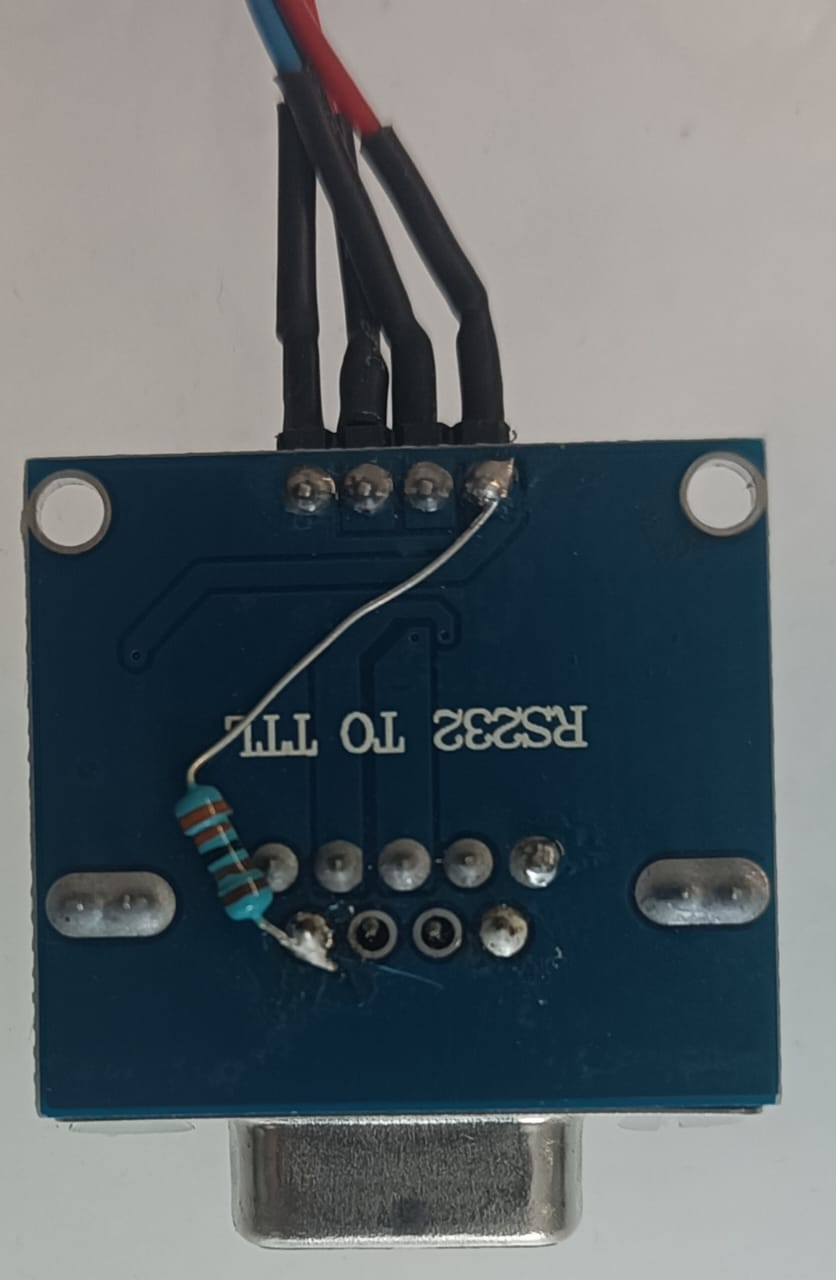
\includegraphics[angle=90, width=0.5\textwidth]{img/RS232_connector.jpeg}
          \caption{Picture of MAX3232 with 3.5kOhm pull-up resistor.}
          \label{MAX3232}
    \end{figure}

Some code that successfully enables communication between an Arduino DUE and the multimeter can be found in the project under 'References/Code that worked'. This is useful to test initial communication with the multimeter. The connections of the Arduino DUE and the MAX3232 module are as shown in Figure\ref{MAX3232_Arduino}.

\begin{figure}[H]
          \centering
          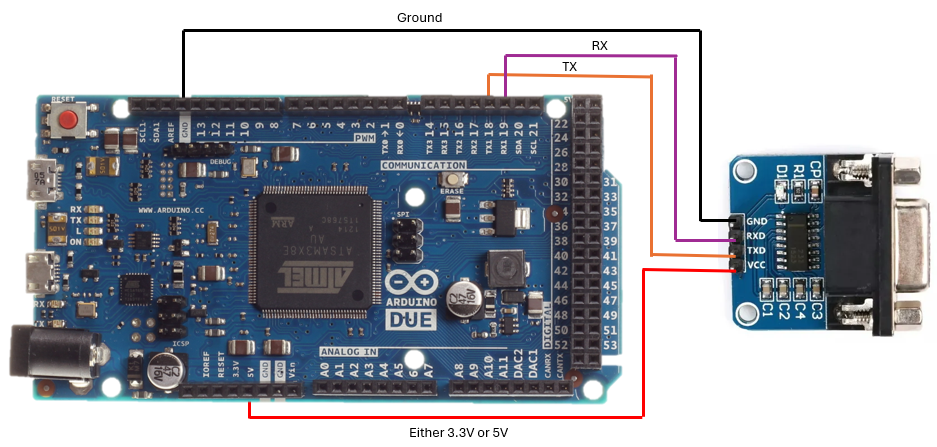
\includegraphics[width=1\linewidth]{img/MAX3232_connection.png}
          \caption{Electrical connection of Arduino DUE and MAX3232.}
          \label{MAX3232_Arduino}
    \end{figure}


\subsection{PCB version 1}
After some rough prototyping the first version of the PCB was developed. The kiCAD design is stored in the project as PCB attempt1. The Arduino program used on it to test its functionality is saved in the project as PCB programming.

\subsection{Another Project Component}
\lipsum[1]